% !TEX encoding = UTF-8 Unicode
%%% Template originaly created by Karol Kozioł (mail@karol-koziol.net) and modified for ShareLaTeX use
\documentclass[a4paper,11pt]{article}
\usepackage[french]{babel} % English language/hyphenation
\usepackage{mathptmx} % Use the Adobe Times Roman as the default text font together with math symbols from the Sym­bol, Chancery and Com­puter Modern fonts

\usepackage[T1]{fontenc}
\usepackage{ucs}
\usepackage[utf8x]{inputenc}
\usepackage{lipsum} % Inserts dummy text
\usepackage{graphicx}
\usepackage{color}

\renewcommand\familydefault{\sfdefault}
\usepackage{tgheros}
%\usepackage[defaultmono]{droidmono}

\usepackage{amsmath,amsfonts,amssymb,amsthm} % For math equations, theorems, symbols, etc
\usepackage{enumerate}
\usepackage{multicol}
\usepackage{tikz}
\usepackage[tikz]{bclogo}
\usepackage{multicol}
\usepackage{geometry}
\geometry{total={210mm,297mm},
left=25mm,right=25mm,%
bindingoffset=0mm, top=20mm,bottom=20mm}
\usepackage{url}
\usepackage[linkbordercolor=blue]{hyperref}
\author{Dr. A. Ammar - IPEST : HAP}
\date{29 janvier 2021}
\setlength{\parindent}{0pt}



\linespread{1.3}

\newcommand{\linia}{\rule{\linewidth}{0.5pt}}

% custom theorems if needed
\newtheoremstyle{mytheor}
    {1ex}{1ex}{\normalfont}{0pt}{\scshape}{.}{1ex}
    {{\thmname{#1 }}{\thmnumber{#2}}{\thmnote{ (#3)}}}

\theoremstyle{mytheor}
\newtheorem{defi}{Definition}

% my own titles
\makeatletter
\renewcommand{\maketitle}{
\begin{center}
\vspace{2ex}
{\huge \textsc{\@title}}
\vspace{1ex}
\\
\linia\\
\@author \hfill \@date
\vspace{4ex}
\end{center}
}
\makeatother
%%%

% custom footers and headers
\usepackage{fancyhdr}
\pagestyle{fancy}
\lhead{}
\chead{}
\rhead{}
\lfoot{}
\cfoot{}
\rfoot{Page \thepage}
\renewcommand{\headrulewidth}{0pt}
\renewcommand{\footrulewidth}{0pt}

%%%%%%%%%%%%%%%%%%%%%%%%%%%%%%%%%%%%%%%%
%%%%%%%%%%%%%%%%%%%%%%%%%%%%%%%%%%%%%%%%%
%%%% CODE
%%%%%%%%%%%%%%%%%%%%%%%%%%%%%%%%%%%%%%%%
\usepackage{fancyvrb} % packages needed for verbatim environments
\usepackage{listingsutf8}

\definecolor{mygreen}{rgb}{0,0.6,0}
\definecolor{mygray}{rgb}{0.5,0.5,0.5}
\definecolor{mymauve}{rgb}{0.58,0,0.82}
\DeclareFixedFont{\ttb}{T1}{pcr}{bx}{n}{10} % for bold
\DeclareFixedFont{\ttm}{T1}{pcr}{m}{n}{10}  % for normal
\lstset{ 
	backgroundcolor=\color{lightgray!10},   % choose the background color; you must add \usepackage{color} or \usepackage{xcolor}; should come as last argument
	basicstyle=\ttm,        % the size of the fonts that are used for the code
	breakatwhitespace=false,         % sets if automatic breaks should only happen at whitespace
	breaklines=true,                 % sets automatic line breaking
	postbreak=\raisebox{0ex}[0ex][0ex]{\ensuremath{\color{red}\hookrightarrow\space}},
	captionpos=b,                    % sets the caption-position to bottom
	commentstyle=\color{mygreen},    % comment style
	deletekeywords={...},            % if you want to delete keywords from the given language
	escapeinside={\%*}{*)},          % if you want to add LaTeX within your code
	extendedchars=true,              % lets you use non-ASCII characters; for 8-bits encodings only, does not work with UTF-8
	firstnumber=1,                % start line enumeration with line 1000
	frameround=fttt,
	frame=single,	                   % adds a frame around the code
	keepspaces=true,                 % keeps spaces in text, useful for keeping indentation of code (possibly needs columns=flexible)
	keywordstyle=\ttb\color{blue},       % keyword style
	language=Python,                 % the language of the code
	morekeywords={*,...},            % if you want to add more keywords to the set
	numbers=left,                    % where to put the line-numbers; possible values are (none, left, right)
	numbersep=5pt,                   % how far the line-numbers are from the code
	numberstyle=\tiny\color{mygray}, % the style that is used for the line-numbers
	rulecolor=\color{black},         % if not set, the frame-color may be changed on line-breaks within not-black text (e.g. comments (green here))
	showspaces=false,                % show spaces everywhere adding particular underscores; it overrides 'showstringspaces'
	showstringspaces=false,          % underline spaces within strings only
	showtabs=false,                  % show tabs within strings adding particular underscores
	stepnumber=1,                    % the step between two line-numbers. If it's 1, each line will be numbered
	stringstyle=\color{mymauve},     % string literal style
	tabsize=4,	                   % sets default tabsize to 2 spaces
	title=\lstname                   % show the filename of files included with \lstinputlisting; also try caption instead of title
}
\usepackage{textcomp}
\DefineVerbatimEnvironment % create new one
{pyshell}{Verbatim}{frame=leftline, framerule=1.5mm, rulecolor=\color{blue}}
\begin{document}
	
\title{Épreuve d'informatique (Python) \textnumero 2 \\ Durée : \texttt{2h}}

\maketitle
\begin{bclogo}[logo=\bcattention, couleurBarre=red, noborder=true, couleur=red!10]{Documents non autorisés.}
\begin{itemize}
\item L'épreuve comporte 3 pages.
\item La présentation, la lisibilité, la qualité de la rédaction et la précision des raisonnements entreront pour une part importante dans l'appréciation des copies.
\item  Les algorithmes doivent être commentés.
\end{itemize}

\end{bclogo}
\section*{Exercice 1 : Générer des coordonnées équidistantes}
Nous voulons générer $n + 1$ coordonnées $x$ équidistantes dans $[a, b]$.\\
Stocker, pour \texttt{a = -2}; \texttt{b = 3} et \texttt{n= 20} les coordonnées $x$ dans une liste \texttt{xList}.


\begin{itemize}
\item[\textbf{Q1.}] Définir toutes les variables puis utiliser une boucle \textbf{for} et ajouter chaque coordonnée à la liste \texttt{xList} (\emph{initialement vide}).

\begin{bclogo}[logo=\bclampe, couleurBarre=green, noborder=true, couleur=yellow!10]{Indications.}
Avec $n$ intervalles, correspondant à $n + 1$ points, dans $[a, b]$, chaque intervalle a une longueur $h = (b-a) / n$. Les coordonnées peuvent alors être générées par la formule \texttt{xi = a + i * h}; $i = 0,…, n$.

\end{bclogo}

\item[\textbf{Q2.}] Utiliser une liste de compréhension comme une implémentation alternative.


\item[\textbf{Q3.}] Vectoriser la liste résultante \texttt{xList} en un tableau numpy \verb|xVect|. \\
N'oubliez pas \textbf{d'importer} d'abord la fonction qui transforme les listes en tableaux à partir de \texttt{numpy}.
\end{itemize}
\section*{Exercice 2 : Courbes paramétriques}
Écrire les programmes Python qui tracent les courbes $y = f(x)$ suivantes:
\begin{enumerate}
\item[\textbf{Q1.}] La Lemniscate de Bernoulli $
\left\{
\begin{array}{ll}
x(t) = \dfrac{sin(t)}{1 + cos^2(t)}&\\
y(t) =\dfrac{sin(t) \times cos(t)}{1 + cos^2(t)}&
\end{array} 
\right.$ 
pour $ t\in[0, 2\pi]$.
\item[\textbf{Q2.}] La spirale d'Archimède $
\left\{
\begin{array}{ll}
x(t) = t \times cos(t)&\\
y(t) =t \times sin(t)&
\end{array} 
\right.$ 
pour $ t\in[0, 10\pi]$.
\newpage
\item[\textbf{Q3.}] La courbe du c\oe{}ur $
\left\{
\begin{array}{ll}
x(t) = 6 \times sin^3(t)&\\
y(t) = cos(t)-5 \times cos(2t)-2 \times cos(3t)-cos(4t)&
\end{array} 
\right.$ 
pour $ t\in[0, 2\pi]$.
\item[\textbf{Q4.}] Les cyclo-harmoniques $
\left\{
\begin{array}{ll}
x(t) = \left( 1 + cos(\dfrac{p}{q}t)\right) \times cos(t) &\\
y(t) = \left( 1 + cos(\dfrac{p}{q}t)\right) \times sin(t)&
\end{array} 
\right.$ 
pour $p$ et $q$ entiers positifs et $ t\in[0, 2\pi]$.
\end{enumerate}
\section*{Exercice 3 : Implémenter une fonction gaussienne}
\begin{itemize}
\item[\textbf{Q1.}] Créer la fonction: \texttt{gauss(x, m = 0, s = 1)}, qui modélise la gaussienne:
\begin{equation*}
f(x) =
{1\over\sqrt{2\pi }\, s}
\exp{\left[-\frac{1}{2}\left({x-m\over s}\right)^2\right]}
\end{equation*}


\item[\textbf{Q2.}] Créer un tableau \texttt{x} à l'aide de la fonction \texttt{linspace}, du module \texttt{numpy}, pour \texttt{100} valeurs \texttt{x} uniformément espacées dans [-10, 10].

\item[\textbf{Q3.}] Écrire les instructions pour tracer le graphique ci-dessous à l'aide de la bibliothèque \texttt{matplotlib}.
\begin{figure}[th!]
\centering
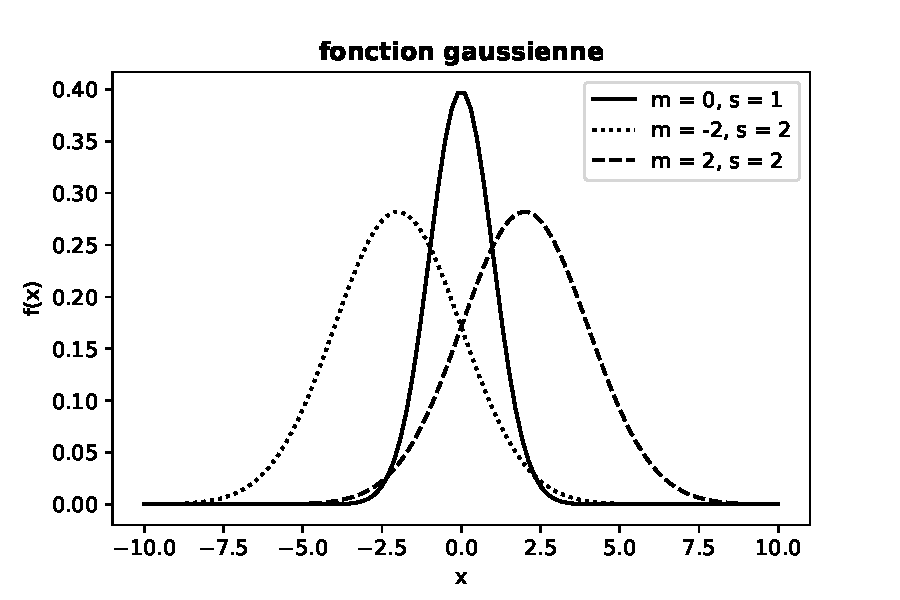
\includegraphics[width=0.9\linewidth]{figures/gaussian}
\label{fig:gaussian}
\end{figure}

\end{itemize}

\section*{Exercice 4 : La suite logistique}
Soit $r$ un réel de $[0,4]$. On considère la suite logistique définie par
$$u_{n+1}=r \times u_n(1-u_n)  \quad et \ u_0= 0.5$$.
Cette suite très célèbre permet de modéliser certaines dynamiques de population. Elle a un comportement très différent selon les valeurs de $r$. On se propose de tracer le nuage de points suivants.
\begin{itemize}
\item[\textbf{Q1.}] Écrire une fonction \verb|Liste_suite(u0,r,n)| qui renvoie la liste des $n$ premiers termes de la suite.

\item[\textbf{Q2.}] Créer une subdivision uniforme \verb|R| de l'intervalle $[0,4]$ en 101 points.
\item[\textbf{Q3.}] Pour chaque élément $r$ de \verb|R|, représenter les points de coordonnées $(r, u_{100})$,$(r, u_{101})$,\dots,$(r, u_{200})$.
\begin{figure}[th!]
\centering
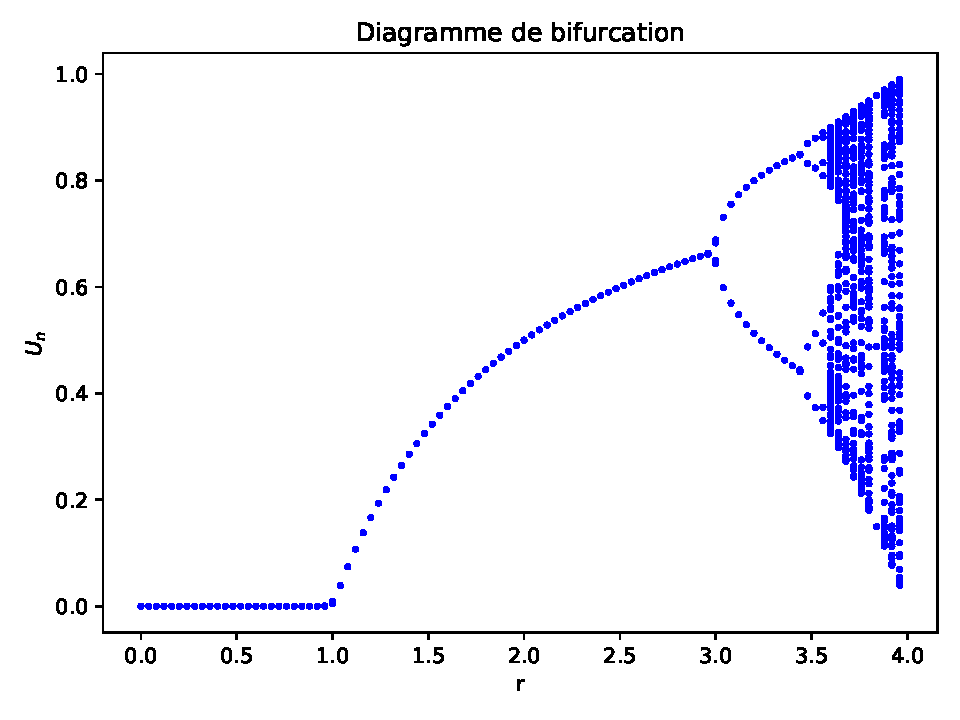
\includegraphics[width=0.9\linewidth]{scripts/bifurcation}
\label{fig:bifurcation}
\end{figure}

\end{itemize}

%\begin{bclogo}[logo=\bclampe, couleurBarre=green, noborder=true, couleur=yellow!10]{Indications.}
%\begin{itemize}
%\item[$\bullet$] `X,Y = np.meshgrid(x,y)`, avec \verb|x| et \verb|y| sont deux tableaux \verb|numpy|, est très utile pour évaluer des fonctions sur une grille.
%\item[$\bullet$] \verb|plt.imshow(X)| afficher une image, à savoir des données sur une trame régulière 2D.
%\end{itemize}
%\end{bclogo}
\end{document}
